\section{Introduction}\label{sec:intro}

\begin{equation}\label{eq:tf}
	H \left( s \right) = K { s - z \over s - p }
\end{equation}

\begin{figure}[tbph]
\centering
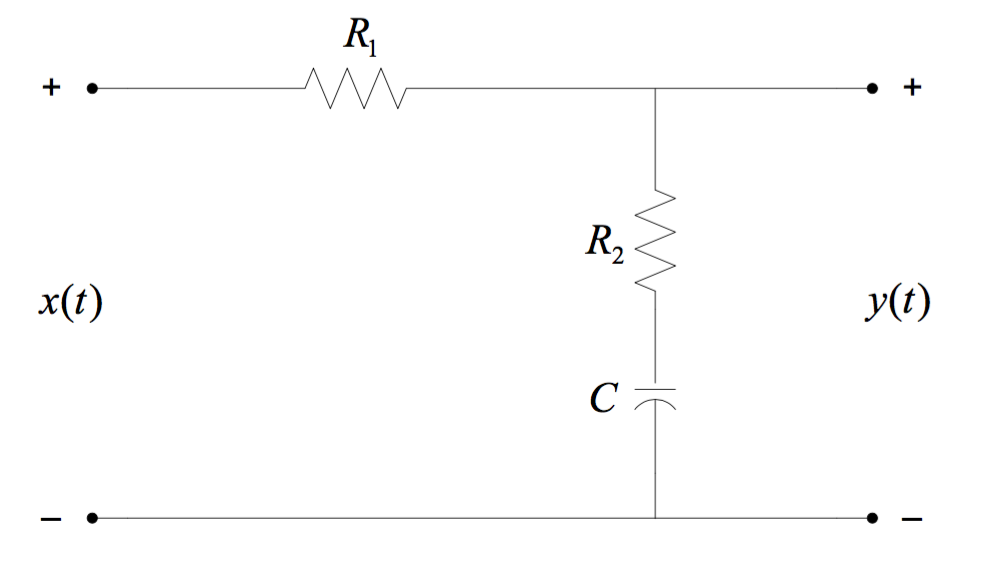
\includegraphics[width=0.7\linewidth]{graphics/lag-schematic}
\caption{Schematic of a phase lag circuit}
\label{fig:schematic}
\end{figure}
For the circuit in Fig. \ref{fig:schematic}, the transfer function is:
\begin{equation}\label{eq:tf-phaselag}
H \left( s \right) = { R_2 + \frac{1}{sC} \over R_1 + R_2 + \frac{1}{sC}} = {R_2 \over R_1 + R_2 } { s + \frac{1}{C R_2} \over s + \frac{1}{C \left( R_1 + R_2 \right)} }.
\end{equation}
Comparing \eqref{eq:tf} with \eqref{eq:tf-phaselag} gives:
\begin{align*}
K &= {R_2 \over R_1 + R_2 } \\
\left|z\right| &= \frac{1}{C R_2} \\
\left|p\right| &= \frac{1}{C \left( R_1 + R_2 \right)}.
\end{align*}
